\chapter{Contexto y estado del arte}

\section{Procesamiento de imágenes satelitales}
    
    El procesamiento de imágenes satelitales desempeña un papel clave en la observación terrestre y el monitoreo ambiental. A lo largo de su evolución, este campo ha integrado innovaciones tecnológicas, datos multiespectrales y métodos avanzados, como el aprendizaje profundo, para abordar problemas complejos. En esta sección, se analiza el contexto histórico, los avances tecnológicos, las aplicaciones actuales y las tendencias que enfrentan las tecnologías satelitales, destacando los desafíos que persisten en su desarrollo.

    \subsection{Historia y avances tecnológicos (1970s-1990s)}

        La evolución de los satélites de observación de la Tierra comenzó con hitos como el lanzamiento del \textit{Landsat 1} en 1972, que introdujo imágenes multiespectrales y permitió avances en cartografía y gestión de recursos naturales. Este satélite marcó el inicio de un enfoque sistemático en la observación terrestre, integrando innovaciones como sensores multiespectrales y la adquisición de datos digitales \autocite{wulder2022fifty}.

        Durante las décadas de 1980 y 1990, los avances tecnológicos dieron lugar a sensores más avanzados, como los radiómetros y los radares de apertura sintética (SAR). Satélites como \textit{SPOT} y \textit{ERS} permitieron nuevas aplicaciones en meteorología, oceanografía y monitoreo de regiones polares. Por ejemplo, los sensores SAR demostraron ser efectivos para mapear regiones cubiertas por nubes o en oscuridad prolongada, mientras que los altímetros proporcionaron mediciones precisas de la topografía oceánica \autocite{amani2022remote}. Estos avances sentaron las bases para las capacidades multiesensor actuales.

    \subsection{Constelaciones y democratización del acceso (2000s-Presente)}

        El desarrollo de programas como \textit{Copernicus} y los satélites \textit{Sentinel} marcó un cambio significativo en la democratización del acceso a datos satelitales de alta calidad mediante modelos de datos abiertos. Esto impulsó aplicaciones innovadoras en agricultura de precisión, monitoreo ambiental y planificación urbana, mientras fomentó la participación ciudadana mediante iniciativas de \textit{crowdsourcing} y sensores accesibles \autocite{karagiannopoulou2022data}.

        La integración de constelaciones masivas, como las gestionadas por el servicio de emergencias de \textit{Copernicus}, también ha mejorado la respuesta a emergencias al proporcionar datos críticos en tiempo casi real. Estas iniciativas han optimizado la precisión y alcance de las acciones en todas las fases de gestión de desastres \autocite{denis2016evolution}.
    
        Por otro lado, las constelaciones privadas como \textit{Planet Labs} han transformado la observación terrestre al combinar alta resolución temporal y espacial con análisis avanzados de \textit{big data}. Estas plataformas han facilitado estudios detallados, como el monitoreo de la conectividad hídrica en regiones árticas \autocite{cooley2017tracking}.

        \begin{figure}[H] 
            \caption{\doublespacing \\ \textit{Comparación de las bandas espectrales de satélites de observación terrestre.}} 
            \centering
            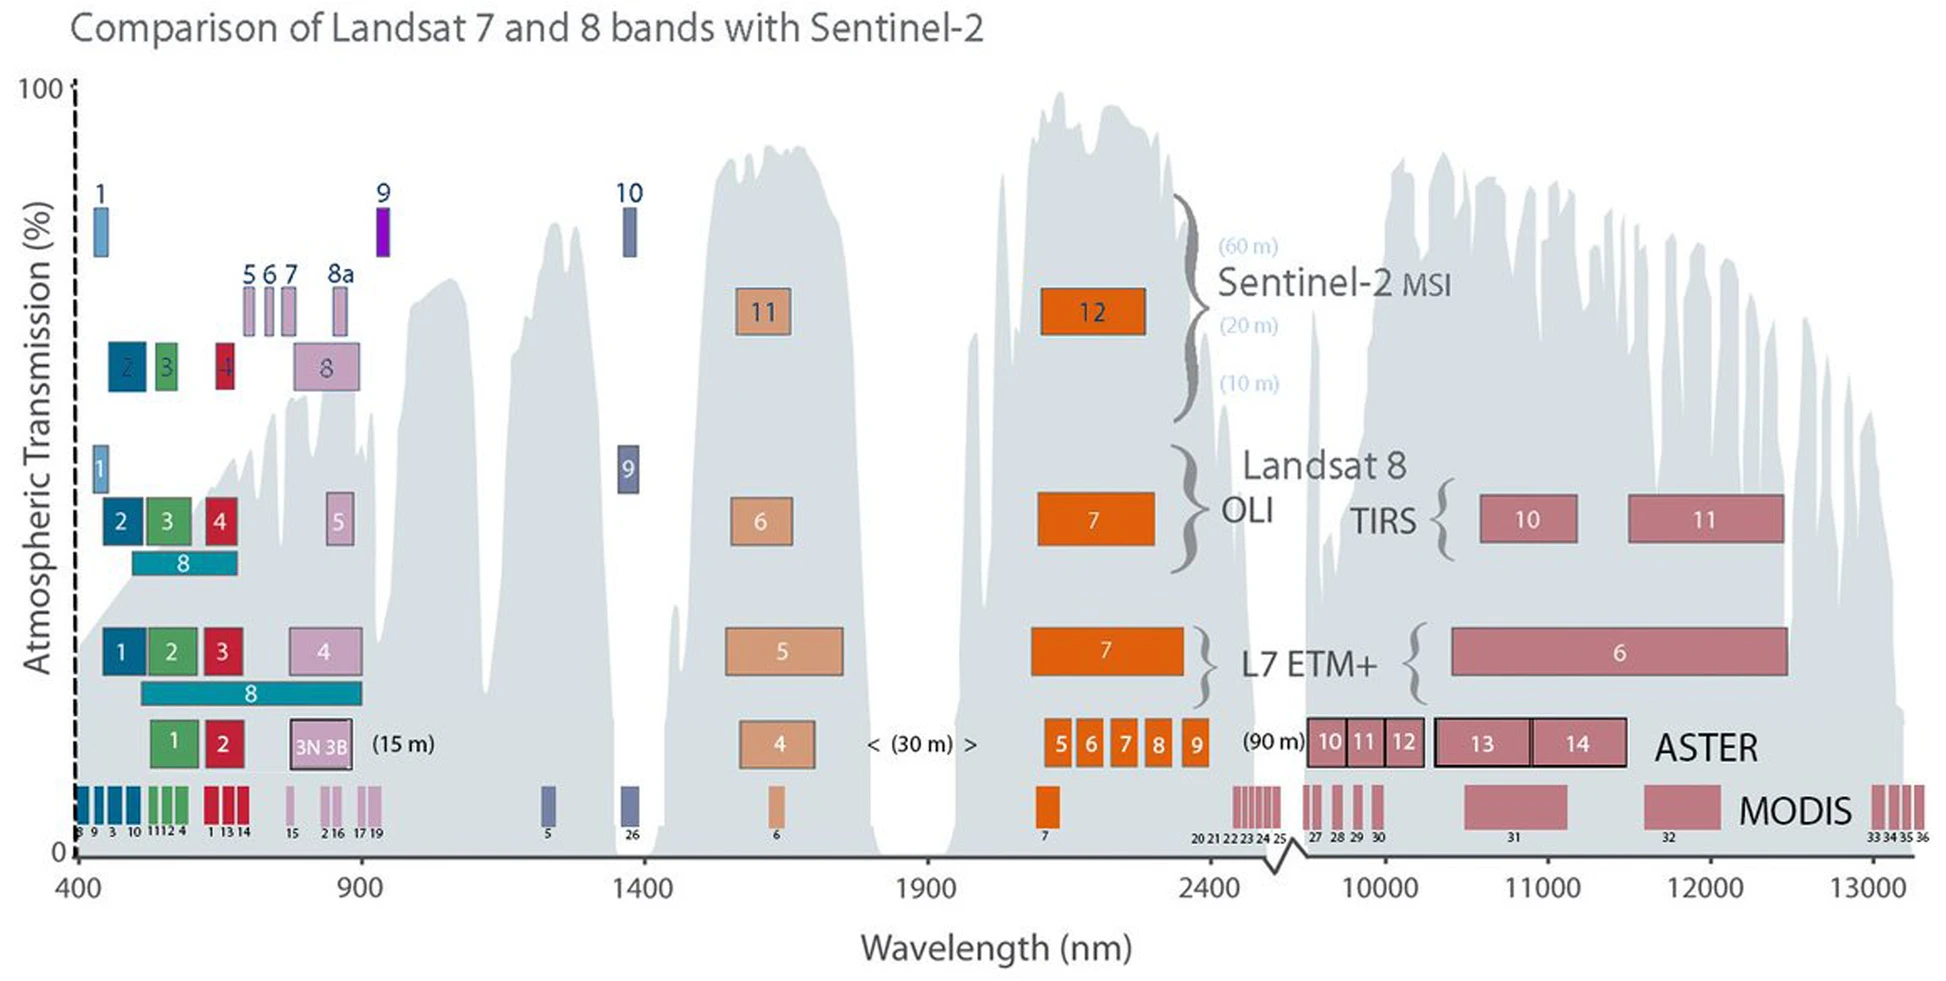
\includegraphics[width=1\linewidth]{images/comparation.png}
            \begin{justify}
                \textit{Nota.} La figura ilustra cómo la diversidad de bandas espectrales en satélites como \textit{Landsat-7}, \textit{Landsat-8} y \textit{Sentinel-2} contribuyen a aplicaciones específicas, como el monitoreo ambiental y la planificación urbana. Recuperado de \textcite{usgslandsat_2016}.
            \end{justify}                    
            \label{fig:comparison}
        \end{figure}

    \subsection{Tendencias actuales y desafíos}

        El futuro del procesamiento de imágenes satelitales está marcado por la miniaturización de satélites, como los CubeSats, y el surgimiento de constelaciones privadas. Los CubeSats, pequeños satélites modulares de $10~\text{cm}^3$, han ampliado el acceso a la observación terrestre al ofrecer alternativas económicas y de fácil implementación. Estas plataformas permiten un monitoreo continuo en regiones remotas y vulnerables, mejorando la capacidad de respuesta ante desastres naturales \autocite{santilli2016disaster}.
        

        \begin{figure}[H] 
            \caption{\doublespacing \\ \textit{Diagrama de Operaciones de la Misión AEROS.}} 
            \centering
            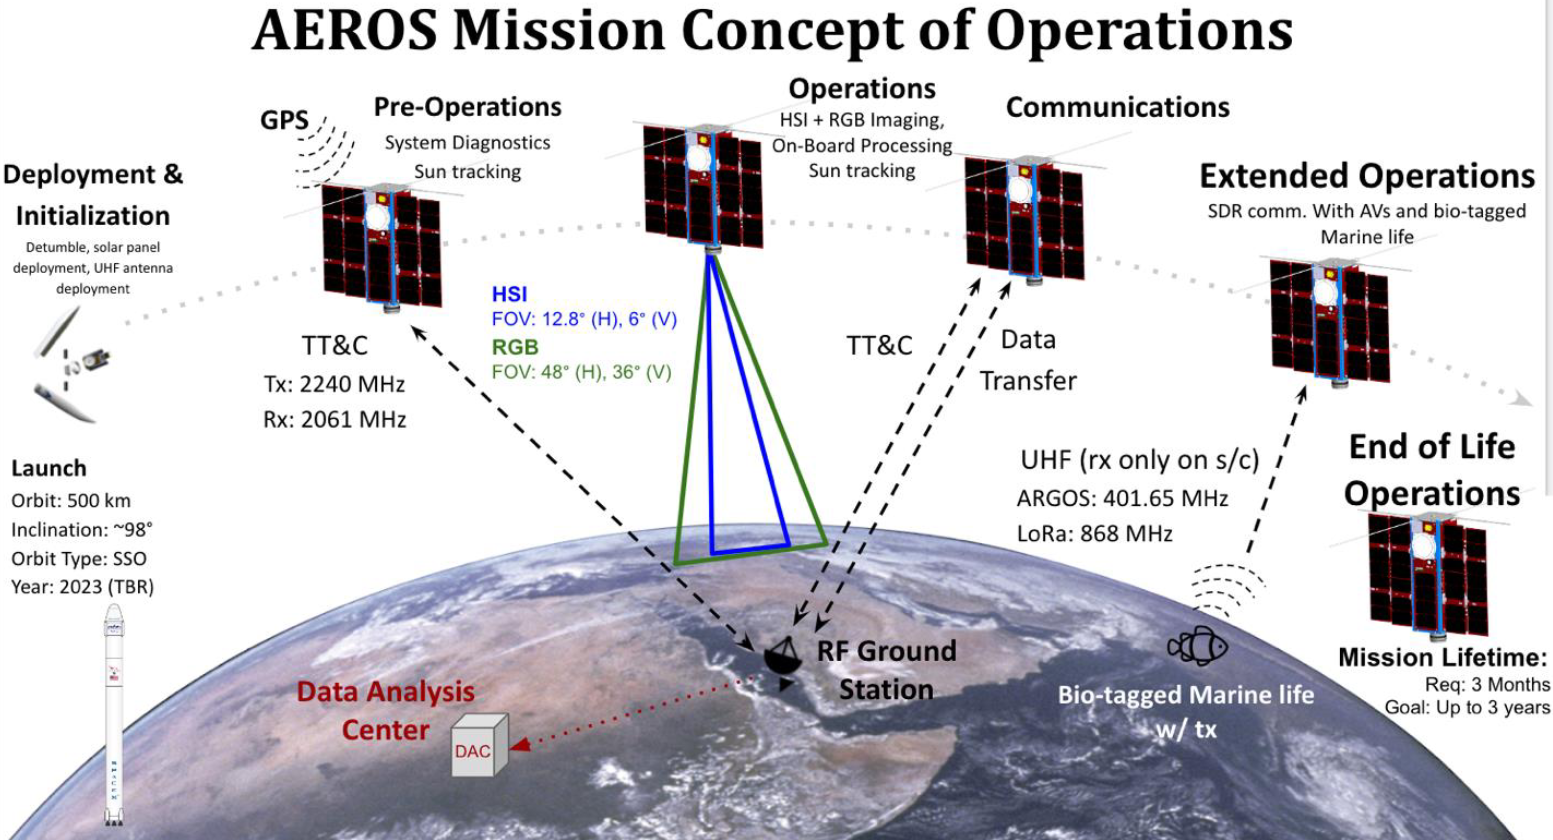
\includegraphics[width=1\linewidth]{images/aeros.png}
            \begin{justify}
                \textit{Nota.} Este diagrama destaca cómo los \textit{CubeSats}, como AEROS, contribuyen al monitoreo ambiental con capacidades avanzadas de adquisición y análisis de datos. Recuperado de \textcite{prendergast2022aeros}.
            \end{justify}                    
            \label{fig:aeros}
        \end{figure}

        Sin embargo, estos avances presentan desafíos como la generación de desechos orbitales, las limitaciones en la miniaturización de sensores y la sostenibilidad financiera. Superar estos obstáculos requiere colaboraciones público-privadas y políticas que promuevan la maniobrabilidad y desorbitación segura \autocite{denis2017towards}.
        

    \subsection{Aplicaciones}
        \subsubsection{Agricultura de precisión}
            La tecnología de imágenes satelitales, proporcionada por sistemas como Sentinel-2 y Landsat, permite monitorear el estado de los cultivos, detectar estrés hídrico y estimar rendimientos agrícolas. Índices espectrales como el NDVI (\textit{Normalized Difference Vegetation Index}) identifican áreas de baja productividad y optimizan el uso de recursos, como agua y fertilizantes \autocite{griffiths2019intra, ed2020recent}. 
            
            Particularmente, un estudio en el sudeste asiático destacó cómo el uso combinado de Sentinel-2 y tecnologías como el SAR optimizó la gestión agrícola bajo diferentes condiciones. Por un lado, índices como el NDVI y el EVI (\textit{Enhanced Vegetation Index}) permitieron reducir el desperdicio de agua en cultivos de arroz en un 20\%, además de ajustar los tiempos de cosecha para maximizar rendimientos. Por otro lado, el SAR facilitó el monitoreo de áreas agrícolas bajo condiciones de nubosidad persistente, complementando los datos ópticos de Sentinel-2 para mejorar el análisis de humedad del suelo y el seguimiento de cultivos en zonas con alta cobertura nubosa \autocite{kaushik2021crop}.
            
        \subsubsection{Gestión de recursos naturales}
            La monitorización de recursos naturales a través de datos satelitales proporciona una supervisión continua de cuerpos de agua, recursos minerales y zonas forestales. Esto facilita estrategias de conservación basadas en evidencia científica. Por ejemplo, el programa Copernicus ha sido clave para evaluar el impacto de la deforestación en la región amazónica, permitiendo la implementación de políticas de reforestación en áreas críticas \autocite{rast2019copernicus}. 
            
            Además, en la gestión de cuencas hidrográficas, la integración de datos satelitales con modelos geoespaciales ha optimizado la toma de decisiones. Un ejemplo notable es el uso combinado de imágenes ópticas y radar para monitorear la calidad del agua en el río Ganges, mejorando la identificación de fuentes de contaminación y el control de flujos hídricos en tiempo real \autocite{caballero2019sentinel, lisboa2024earth}.
            
        \subsubsection{Respuesta a emergencias}
            Las imágenes satelitales de alta resolución, combinadas con datos en tiempo real, son fundamentales para responder a desastres naturales como inundaciones y terremotos. Por ejemplo, durante las inundaciones en el sudeste asiático en 2021, la combinación de datos de Planet Labs y Sentinel permitió identificar áreas afectadas en menos de 48 horas, optimizando la distribución de ayuda humanitaria \autocite{matgen2020feasibility}. 
            
            Una aplicación destacada es el uso de Sentinel-1 para evaluar la extensión de incendios forestales mediante tecnologías de radar, incluso bajo condiciones de humo denso. Este enfoque mejora la precisión del mapeo de áreas quemadas y facilita una planificación efectiva para la recuperación de los ecosistemas \autocite{ajmar2017response}. 
        
    \subsection{Desafíos}
        \subsubsection{Resolución espacial y temporal}
            La precisión de las aplicaciones depende de la resolución espacial y temporal de los datos. Mientras que satélites como Sentinel-2 ofrecen una resolución espacial de 10 metros, esto puede ser insuficiente para análisis detallados, como la detección de cultivos individuales. En contraste, sistemas privados como PlanetScope proporcionan imágenes con resolución de hasta 30 cm por píxel, aunque su alto costo sigue siendo una barrera para su adopción generalizada \autocite{schiavon2021monitoring}.
        
        \subsubsection{Ruido y efectos atmosféricos}
            Los efectos atmosféricos, como la presencia de nubes y aerosoles, afectan la calidad de las imágenes ópticas, reduciendo su utilidad en ciertas aplicaciones. No obstante, tecnologías como el radar de apertura sintética (SAR) ofrecen soluciones robustas frente a estas limitaciones, mejorando el monitoreo en regiones con condiciones climáticas adversas \autocite{caballero2019sentinel}.
        
        \subsubsection{Fusión de datos multisensor}
            Combinar datos ópticos, térmicos y de radar sigue siendo un desafío técnico debido a las diferencias en resoluciones espaciales y espectrales. Sin embargo, estas herramientas están logrando avances importantes, particularmente en aplicaciones agrícolas donde se requiere combinar datos de humedad del suelo con índices espectrales \autocite{rast2019copernicus}.
        

        \subsubsection{Manejo de grandes volúmenes de datos}
            La cantidad de datos generados por satélites modernos plantea retos significativos en almacenamiento y análisis, especialmente en regiones con recursos tecnológicos limitados. Este problema se agrava en estudios que requieren integración de múltiples fuentes \autocite{matgen2020feasibility}.


        \subsubsection{Accesibilidad y costo}
            Aunque programas como Copernicus han mejorado el acceso a datos satelitales, las imágenes de muy alta resolución, ofrecidas por empresas privadas, siguen siendo una barrera económica para su adopción generalizada \autocite{denis2016evolution}.

\section{Armonización de datos}

    La armonización de datos busca garantizar la coherencia entre imágenes satelitales con distintas resoluciones espaciales, espectrales y temporales. Este proceso es esencial para aplicaciones avanzadas en teledetección, como la superresolución y la fusión multiespectral. La armonización establece la base para técnicas avanzadas, como la superresolución, que requieren datos consistentes para lograr precisión en tareas específicas. En esta sección, se analizan los aspectos fundamentales relacionados con las características de la misión Sentinel-2, los conjuntos de datos empleados en el contexto de la superresolución y las técnicas relevantes para mejorar la calidad y utilidad de las imágenes.

    \subsection{La misión Sentinel-2}

        La misión Sentinel-2 forma parte del programa Copernicus liderado por la Agencia Espacial Europea (ESA). Su objetivo principal es proporcionar datos multiespectrales de alta calidad para monitorear los cambios en la superficie terrestre, incluyendo agricultura, forestación, y recursos hídricos. Es clave en la gestión de emergencias y la vigilancia medioambiental gracias a su amplio alcance y frecuencia de revisita \autocite{wang2016fusion, lanaras2018super}.

        \subsubsection{Resolución espacial}
            Proporciona imágenes con resoluciones espaciales de 10, 20 y 60 metros, dependiendo de las bandas espectrales. Las bandas de 10 metros incluyen el visible (RGB), mientras que las bandas de 20 metros abarcan regiones como el infrarrojo cercano (NIR) y el infrarrojo de onda corta (SWIR). Sin embargo, estas bandas de 20 metros, aunque frecuentemente utilizadas para aplicaciones como el monitoreo del agua o la clasificación de cultivos, presentan limitaciones en cuanto al detalle espacial. Para abordar este desafío, se han propuesto soluciones basadas en redes neuronales convolucionales, como FUSE, que generan superresoluciones eficientes al combinar bandas de alta y baja resolución, asegurando la preservación de las características espectrales y estructurales \autocite{gargiulo2019fast}. Además, para aprovechar al máximo las capacidades del sensor, investigaciones recientes han explorado cómo las correlaciones entre bandas de diferente resolución pueden emplearse para mejorar las bandas de 20 y 60 metros a través de técnicas de superresolución basadas en aprendizaje profundo \autocite{lanaras2018super}.

        \subsubsection{Resolución espectral}
            Sentinel-2 abarca 13 bandas espectrales, desde el ultravioleta hasta el infrarrojo de onda corta. Estas bandas permiten una caracterización detallada de la superficie terrestre, incluyendo la detección de cambios en la vegetación, la humedad del suelo y la calidad del agua \autocite{wang2016fusion}.


        \subsubsection{Resolución temporal}

            Compuesta por los satélites Sentinel-2A y Sentinel-2B, la misión ofrece un tiempo de revisita de 5 días, permitiendo una vigilancia casi continua, especialmente útil en estudios dinámicos. Se prevé el lanzamiento de Sentinel-2C en el futuro para ampliar la constelación \autocite{Sentinel2C_Copernicus_2024}. Esto asegurará la continuidad en la adquisición de imágenes y mantendrá la calidad de los datos para una amplia gama de aplicaciones.
        
        \subsubsection{Resolución temporal}

            La misión Copernicus Sentinel-2 actualmente cuenta con tres satélites en órbita: Sentinel-2A, Sentinel-2B y, más recientemente, Sentinel-2C, lanzado el 4 de septiembre de 2024 \autocite{Sentinel2C_Copernicus_2024}. 
            
            Con el lanzamiento de Sentinel-2C, que reemplazará gradualmente a Sentinel-2A, y el futuro Sentinel-2D que tomará el relevo de Sentinel-2B, se garantiza la continuidad de datos esenciales con una cobertura cada cinco días. Este avance fortalece el programa Copernicus en la observación de la Tierra y asegura la sostenibilidad de la misión más allá de 2035 con las futuras misiones Sentinel-2 Next Generation.

        \subsubsection{Niveles de procesamiento}

            Sentinel-2 ofrece imágenes en dos niveles: L1C y L2A \autocite{ginting2024comparison}.
            
            \paragraph{L1C}
            Datos en reflectancia TOA con correcciones geométricas y radiométricas, útiles para análisis generales, pero sin corrección atmosférica. Estas imágenes son adecuadas para estudios espaciales básicos, aunque pueden estar influenciadas por efectos atmosféricos.
            
            \paragraph{L2A}
            Datos BOA corregidos atmosféricamente con Sen2Cor, ideales para estudios precisos como monitoreo de cultivos y agua. Estas imágenes eliminan los efectos de la atmósfera y el terreno, pero pueden presentar sobrecorrecciones en áreas con topografía compleja debido a limitaciones en el modelo de elevación digital (DEM).
            
            \paragraph{Elección}
            \begin{itemize}
                \item \textbf{L1C:} Para análisis espaciales generales sin necesidad de corrección atmosférica.
                \item \textbf{L2A:} Para estudios que requieren alta precisión en reflectancia superficial corregida.
            \end{itemize}
            
            
            
            \begin{table}[H]
                \caption{\doublespacing \\ \textit{Comparación de bandas espectrales de Sentinel-2.}}
                \begin{spacing}{8}
                    \fontsize{10pt}{2pt}\selectfont  
                    \begin{tabularx}{\linewidth}{>{\centering\arraybackslash}P{3.5cm} >{\centering\arraybackslash}P{3.2cm} >{\centering\arraybackslash}P{4.2cm} >{\centering\arraybackslash}P{2.8cm}} 
                        \toprule
                        \textbf{Designación de banda} & \textbf{Resolución (m)} & \textbf{Longitud de onda (nm)} & \textbf{Descripción} \\
                        \midrule
                        B1  & 60 & 443.9--442.3 & Aerosols \\
                        B2  & 10 & 496.6--492.1 & Blue \\
                        B3  & 10 & 560.0--559.0 & Green \\
                        B4  & 10 & 664.5--665.0 & Red \\
                        B5  & 20 & 703.9--703.8 & Red Edge 1 \\
                        B6  & 20 & 740.2--739.1 & Red Edge 2 \\
                        B7  & 20 & 782.5--779.7 & Red Edge 3 \\
                        B8  & 10 & 835.1--833.0 & NIR \\
                        B8A & 20 & 864.8--864.0 & Red Edge 4 \\
                        B9  & 60 & 945.0--943.2 & Water vapor \\
                        B11 & 20 & 1613.7--1610.4 & SWIR 1 \\
                        B12 & 20 & 2202.4--2185.7 & SWIR 2 \\
                        \bottomrule
                    \end{tabularx}
                \end{spacing}
                \vspace{1\baselineskip}
                \textit{Nota.} Comparación de las bandas espectrales, resoluciones espaciales y longitudes de onda del satélite Sentinel-2. Adaptado de \textcite{gargiulo2019fast}.\\
                \label{tab:BandasSentinel}
            \end{table}
            
    \subsection{Conjuntos de datos para superresolución}
        \label{chapter:datasets}
        
        La selección adecuada de conjuntos de datos desempeña un rol esencial en el desarrollo y rendimiento de algoritmos de superresolución. Estos conjuntos presentan una variedad de características, desde resolución espacial y espectral hasta diversidad geográfica, que impactan en la eficacia de los modelos. A continuación, se describen los principales conjuntos de datos utilizados en este ámbito, destacando sus aplicaciones y limitaciones.
        
        \subsubsection{OpenImages}
        
            Diseñado originalmente para tareas de visión por computadora, incluye una vasta colección de imágenes RGB que representan escenas cotidianas. Aunque su contenido no está relacionado directamente con la teledetección, este dataset es valioso para el preentrenamiento de modelos debido a su amplio volumen y accesibilidad bajo licencia CC-BY. Las imágenes de alta resolución (HR) alcanzan hasta 0.5 metros, mientras que las de baja resolución (LR) se generan sintéticamente mediante interpolación para alcanzar dimensiones de 128×128 píxeles.
            
            Pese a las diferencias espectrales y espaciales con respecto a los datos de teledetección, OpenImages ha demostrado ser útil en la transferencia de aprendizaje, permitiendo que modelos preentrenados en este conjunto se ajusten eficazmente a dominios específicos como Sentinel-2 \autocite{gargiulo2019fast}.
            
        
        \subsubsection{NAIP}
        
            El Programa Nacional de Imágenes de Agricultura (NAIP) recopila imágenes aéreas multiespectrales de alta resolución (0.6 metros) en los Estados Unidos. Estas imágenes, utilizadas principalmente para aplicaciones agrícolas, incluyen bandas espectrales como rojo, verde, azul e infrarrojo cercano (NIR). NAIP es un recurso abierto que proporciona datos actualizados regularmente, facilitando análisis detallados en agricultura de precisión y gestión de tierras.
            
            En contextos de superresolución, el NAIP se emplea como referencia para comparar su alta resolución con las imágenes de Sentinel-2, permitiendo validar modelos que buscan mejorar la resolución espacial \autocite{gargiulo2019fast}.
            
            \begin{figure}[H] 
                \caption{\doublespacing \\ \textit{Comparación visual entre Sentinel-2 y NAIP.}} 
                \centering
                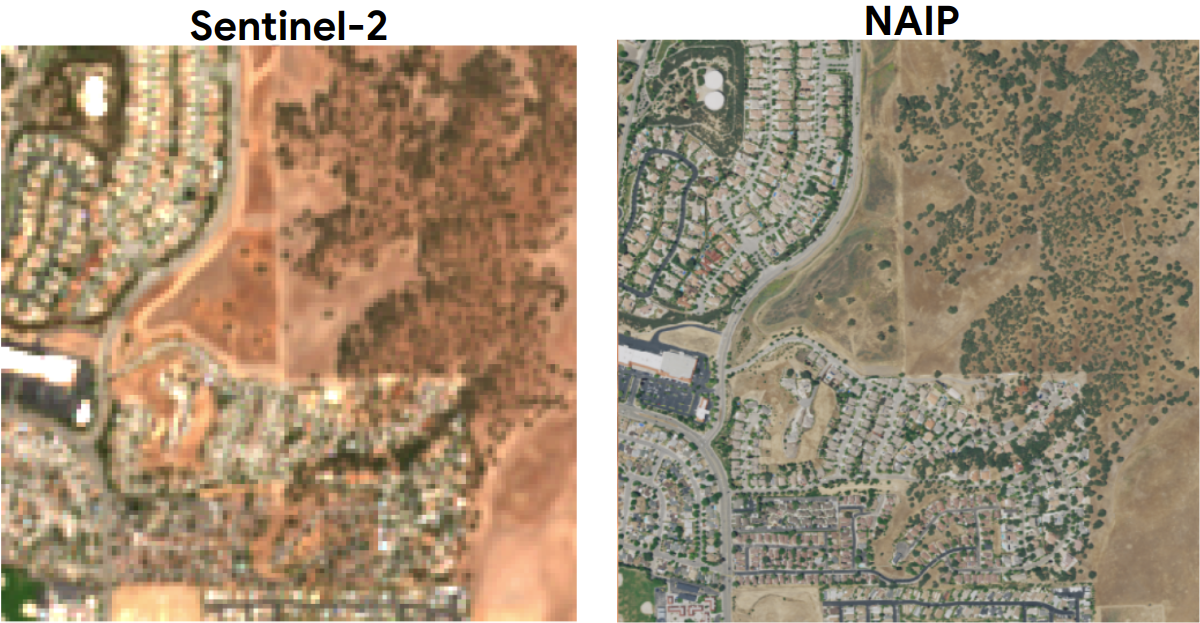
\includegraphics[width=1\linewidth]{images/s2_naip.png}
                \begin{justify}
                    \textit{Nota.} La imagen muestra una comparación entre Sentinel-2 y NAIP. NAIP destaca por su mayor nivel de detalle, mientras que Sentinel-2 proporciona cobertura multiespectral útil para análisis globales y temporales. Elaboración propia.
                \end{justify}                    
                \label{fig:s2_naip}
            \end{figure}

        \subsubsection{Sen2Venus}
        
            El conjunto de datos Sen2Venus está diseñado específicamente para la mejora de resolución espacial de las bandas de Sentinel-2. Este dataset combina imágenes de Sentinel-2 con datos de referencia adquiridos por el satélite VENμS, que proporciona una resolución de 5 metros. Los datos, libres de nubes, abarcan 29 ubicaciones globales con un total de 132,955 parches de 256×256 píxeles.
            
            Sen2Venus es clave para la armonización de datos multiespectrales, permitiendo pruebas directas de algoritmos de superresolución que buscan preservar la coherencia espectral y espacial \autocite{michel2022sen2venmus}.

        
        \subsubsection{Sentinel-2 degradado}
        
            El conjunto Sentinel-2 degradado genera pares sintéticos de imágenes LR-HR en el dominio espectral de Sentinel-2. Las imágenes de alta resolución, originalmente de 10 metros, se degradan mediante un núcleo de convolución para obtener pares con resoluciones de 40 y 10 metros, correspondientes a un factor de superresolución de 4.
            
            Este dataset supera problemas comunes como desajustes geométricos y espectrales, proporcionando una base sólida para entrenar y evaluar modelos de superresolución desde cero. Sin embargo, las diferencias en la frecuencia espacial entre los objetos del suelo y los datos de Sentinel-2 representan un desafío adicional \autocite{wang2016fusion}.
            

            \begin{figure}[H]
                \caption{\doublespacing \\ \textit{Ejemplo del conjunto de datos degradado Sentinel-2 (HR: 10m, LR: 40m).}} 
                \centering
                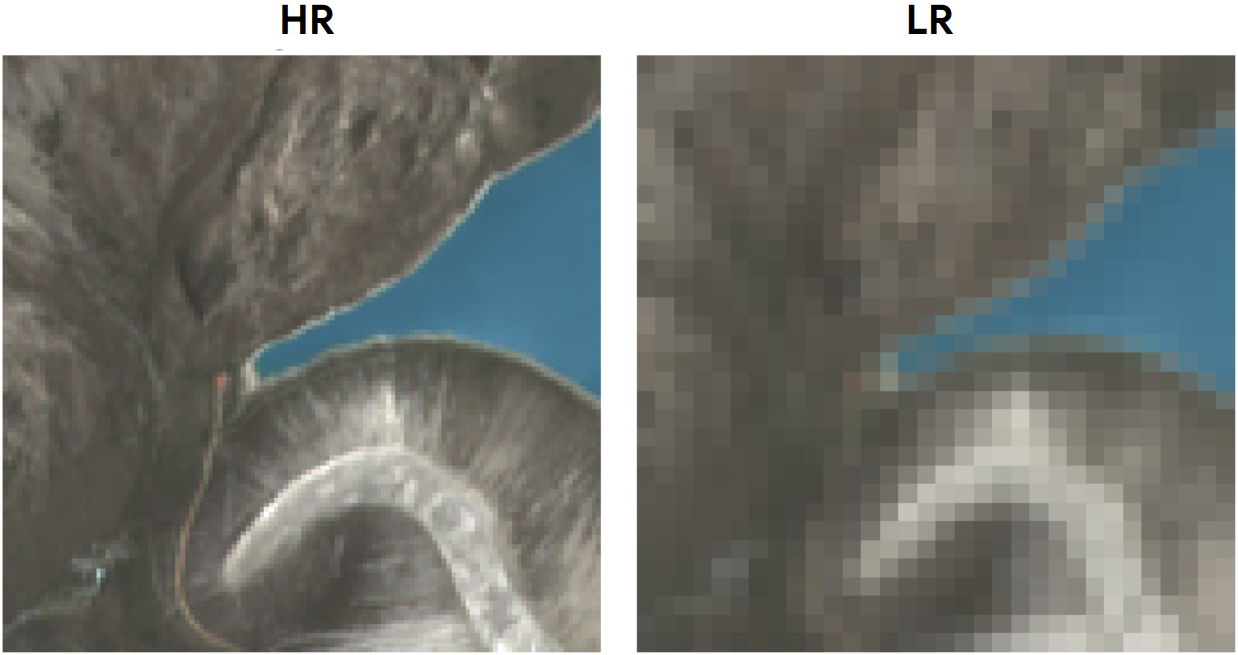
\includegraphics[width=1\linewidth]{images/hr_lr_degraded.png}
                \begin{justify}
                    \textit{Nota.} La figura ilustra la degradación de una imagen de alta resolución (HR) a baja resolución (LR) mediante un núcleo de convolución. Este proceso se utiliza comúnmente en el desarrollo de algoritmos de superresolución para entrenar modelos capaces de restaurar detalles espaciales a partir de datos degradados. Elaboración propia.
                \end{justify}                    
                \label{fig:hr_lr_degraded}
            \end{figure}
            
    \subsection{Resolución Espacial Efectiva}

        La resolución espacial efectiva es un parámetro fundamental en la calidad de las imágenes satelitales, ya que refleja la capacidad del sistema de capturar detalles espaciales más allá de las limitaciones geométricas del píxel. Aunque a menudo se relaciona directamente con el tamaño del píxel (GSD, \textit{Ground Sampling Distance}), su definición práctica depende de factores como las propiedades ópticas del sistema y la dispersión de la energía luminosa en los píxeles, representada por la PSF (\textit{Point Spread Function}).
        
        \begin{itemize}
            \item \textbf{Propiedades ópticas del sistema:} Elementos como la apertura del lente y la longitud focal determinan la cantidad de detalles que pueden capturarse, influenciando directamente la resolución espacial efectiva \autocite{valenzuela2022new}.
            \item \textbf{PSF (Point Spread Function):} Describe cómo la energía de una fuente puntual se distribuye entre varios píxeles. La PSF no solo modela las limitaciones geométricas, sino que también evalúa la calidad del sistema en términos de precisión óptica y electrónica \autocite{pampanoni2024analysing}.
        \end{itemize}
        
        En este contexto, la resolución espacial efectiva puede describirse en términos de diferentes configuraciones de muestreo, basadas en el parámetro \( Q \), que representa la relación entre el tamaño del píxel y la extensión de la PSF:
        
        \begin{itemize}
            \item \textbf{Bajo muestreo (\( Q < 0.7 \)):} La señal se dispersa significativamente, perdiendo detalles espaciales críticos.
            \item \textbf{Muestreo óptimo (\( 0.7 \leq Q \leq 1.5 \)):} Logra un equilibrio entre el tamaño del píxel y la dispersión de la señal, maximizando la resolución efectiva.
            \item \textbf{Sobre-muestreo (\( Q > 1.5 \)):} Aunque preserva los detalles, puede resultar en un uso ineficiente de los recursos de almacenamiento y procesamiento.
        \end{itemize}

        \begin{figure}[H]
            \caption{\doublespacing \\ \textit{Distribución de la PSF y su impacto en la resolución espacial efectiva.}} 
            \centering
            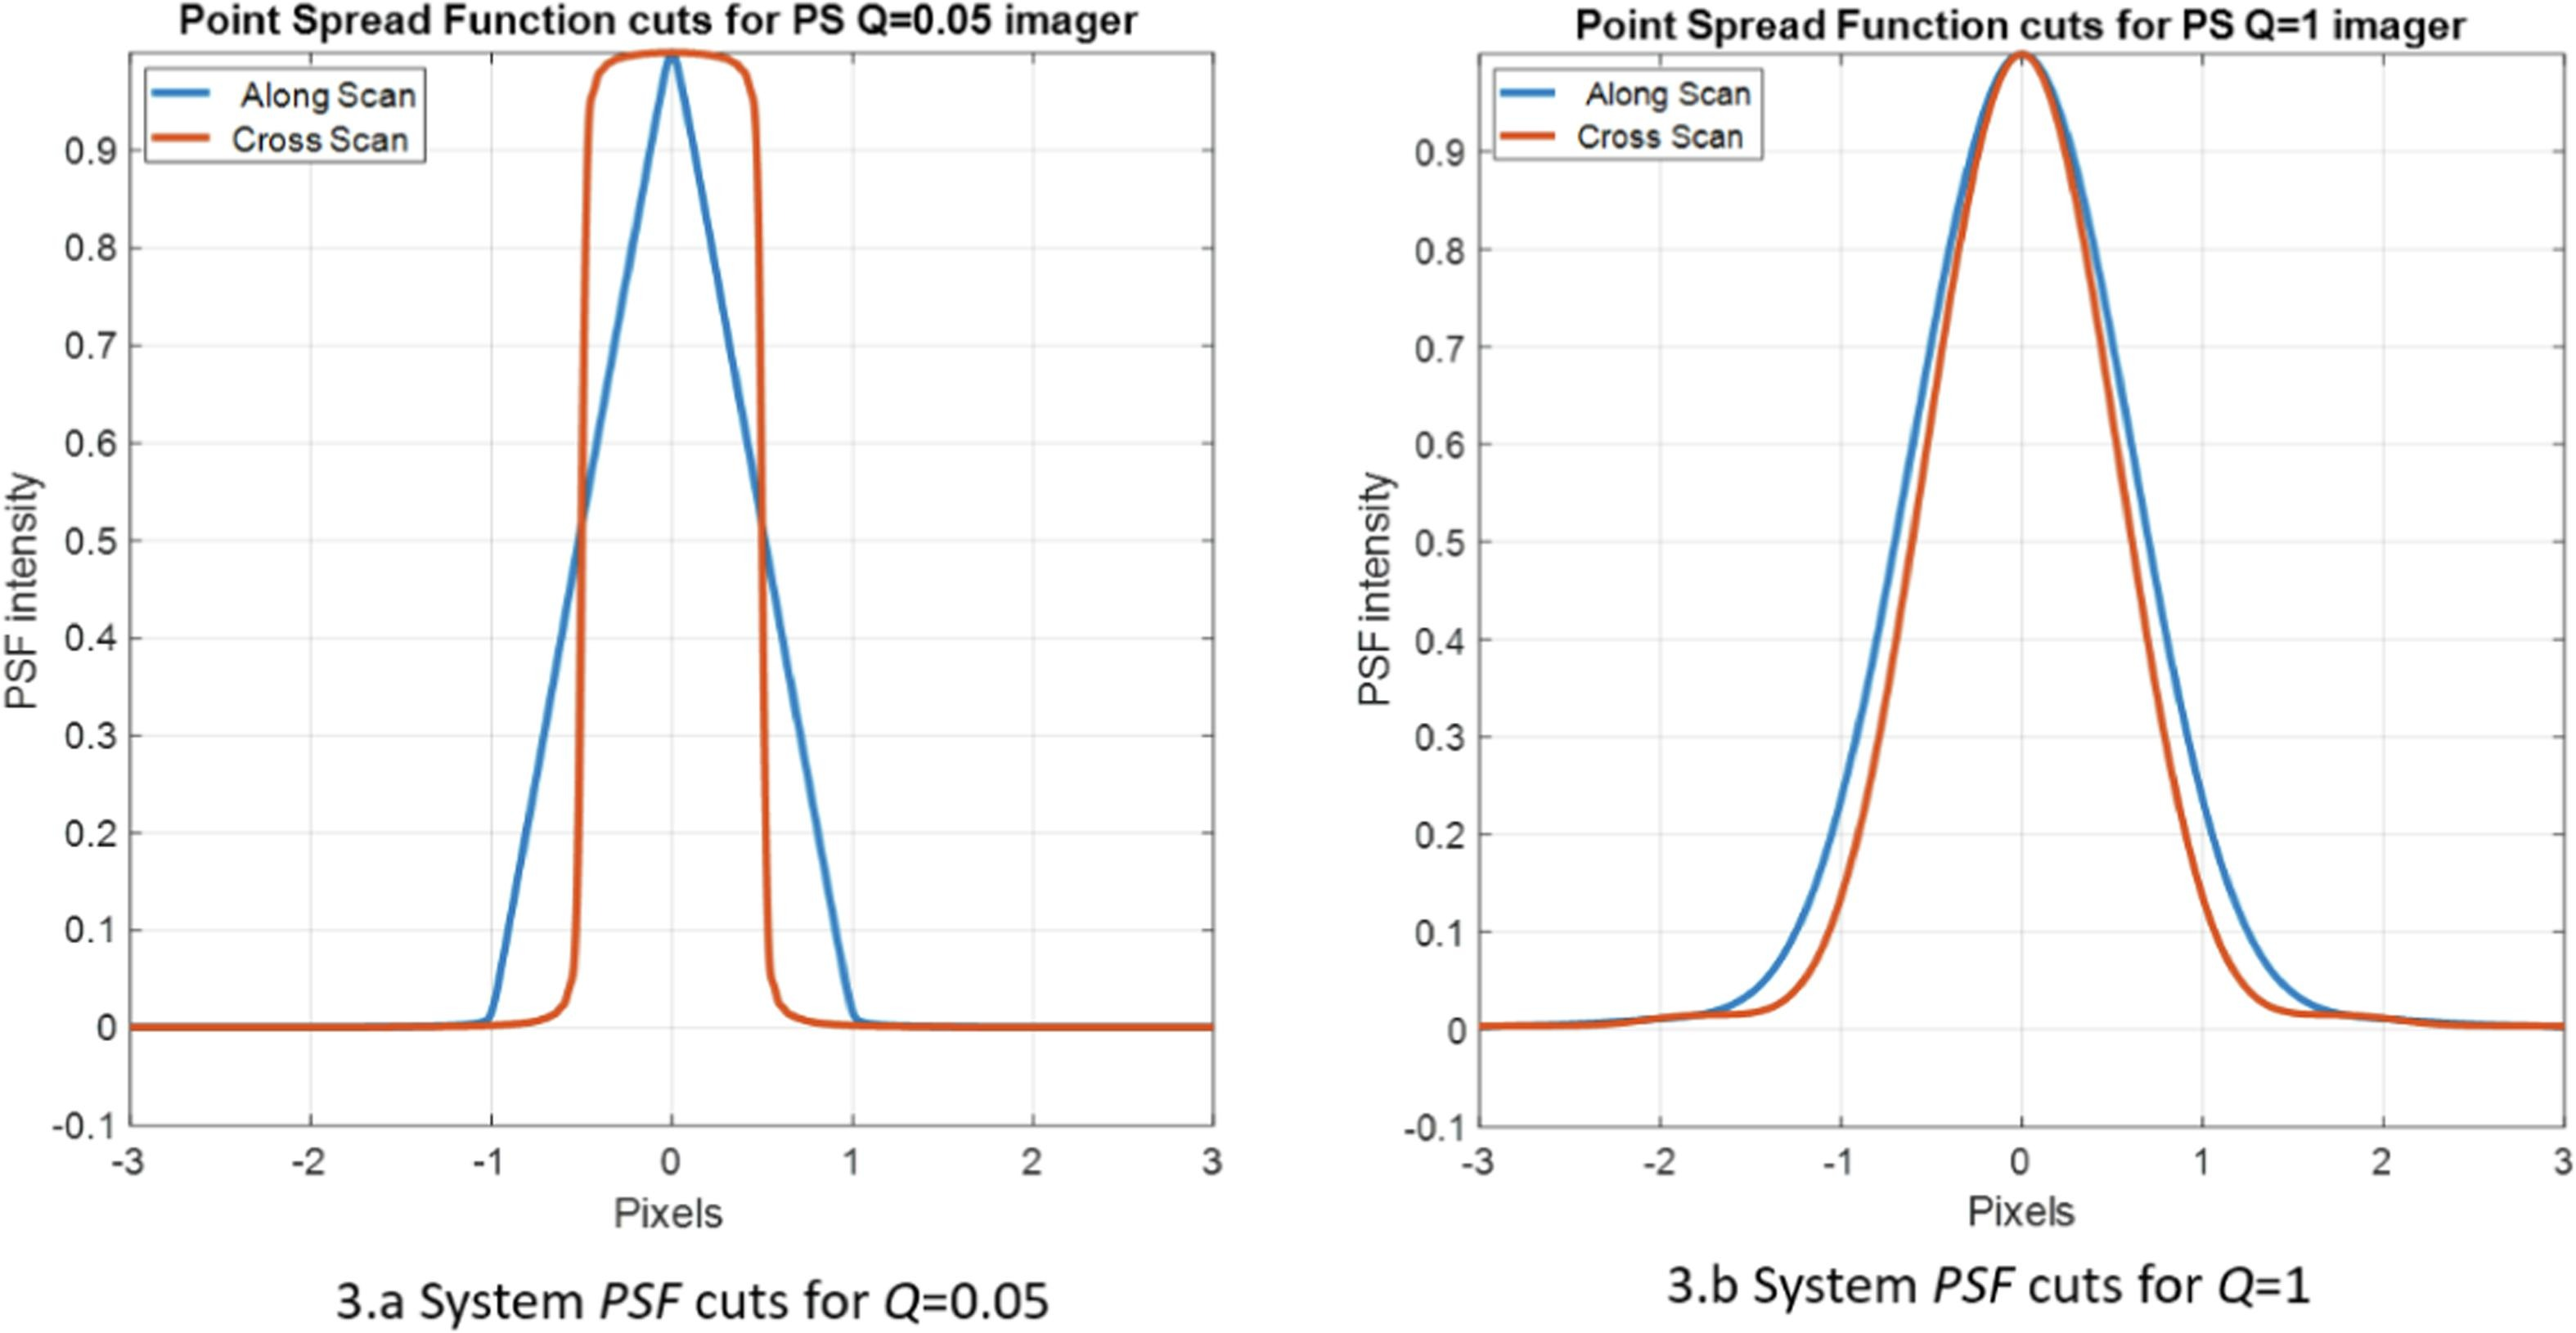
\includegraphics[width=1\linewidth]{images/psf.jpg}
            \begin{justify}
                \textit{Nota.} Distribución de la PSF en las direcciones Along Scan y Cross Scan para condiciones de muestreo insuficiente (\( Q = 0.05 \)) y óptimo (\( Q = 1 \)), mostrando cómo se afecta la preservación de detalles espaciales. Recuperado de \textcite{valenzuela2022new}.
            \end{justify}                    
            \label{fig:psf}
        \end{figure}
        

        Este análisis subraya la importancia de optimizar el diseño del sistema para alcanzar un equilibrio entre resolución geométrica y calidad óptica. Este concepto conecta directamente con la evaluación de la MTF (\textit{Modulation Transfer Function}), ya que esta permite comprender cómo las frecuencias espaciales se preservan en el proceso de captura de imágenes.
        
        \subsubsection{Modulation Transfer Function (MTF)}
            
            Es una métrica clave para evaluar cómo un sistema óptico o sensor de imágenes preserva las frecuencias espaciales, desde patrones más amplios hasta detalles finos. Se determina mediante la Transformada de Fourier de la Función de Dispersión de Punto (PSF), y se define como:

            \[
            \text{MTF}(f) = |\mathcal{F}\{\text{PSF}(x, y)\}|
            \]
            
            Donde:
            \begin{itemize}
                \item \( f \): frecuencia espacial medida en ciclos por unidad de distancia.
                \item \( \mathcal{F} \): Transformada de Fourier de la PSF.
                \item \( \text{PSF}(x, y) \): representación espacial de la dispersión de luz para una fuente puntual.
            \end{itemize}
            
            Un valor alto en la MTF indica una alta capacidad para transmitir detalles de alta frecuencia espacial, mientras que valores bajos sugieren una pérdida de resolución y disminución de nitidez. Estudios recientes han demostrado que las técnicas basadas en la MTF son fundamentales para mejorar la calidad de imágenes satelitales, como las de Sentinel-2, al incorporar modelos de degradación que reflejan fielmente la capacidad del sensor para capturar diferentes rangos de frecuencias espaciales \autocite{hubble2021single}.
            
        \subsubsection{MTF en Sentinel-2}

            En el caso del satélite Sentinel-2, la \textit{Modulation Transfer Function} (MTF) varía dependiendo de las bandas espectrales, reflejando diferencias en la capacidad de captura de detalles espaciales:
            
            \begin{itemize}
                \item \textbf{Bandas de 10 m:} Caracterizadas por una MTF alta, son ideales para capturar detalles finos, especialmente en aplicaciones como el monitoreo urbano y agrícola.
                \item \textbf{Bandas de 20 m:} Con una MTF moderada, logran un balance entre resolución espacial y área cubierta, siendo útiles para estudios de vegetación.
                \item \textbf{Bandas de 60 m:} Diseñadas para observaciones a gran escala, estas bandas priorizan patrones generales, lo que resulta en una MTF más baja pero adecuada para análisis globales.
            \end{itemize}
            
            Estudios recientes han demostrado que el diseño de Sentinel-2, que utiliza valores específicos de MTF adaptados a cada banda espectral, asegura una optimización de las aplicaciones según las necesidades de resolución espacial y espectral \autocite{donike2022deep}.
            
        
        \subsubsection{MTF y fusión de imágenes}

            En el proceso de fusión de imágenes de diferentes bandas y resoluciones, la \textit{Modulation Transfer Function} (MTF) desempeña un papel esencial al balancear las frecuencias espaciales altas y bajas. Las bandas de mayor resolución contribuyen con detalles finos, mientras que las de menor resolución aportan información contextual, formando una representación integrada y coherente. La MTF garantiza que las propiedades espaciales y espectrales de cada banda se conserven durante la integración. Un análisis reciente demostró que métodos de fusión basados en MTF logran una alta fidelidad espacial y espectral al ajustar las diferencias inherentes en la resolución de sensores como Sentinel-2 y otros sistemas multiespectrales \autocite{zhu2024fusion}.
            
        
        \subsubsection{MTF y modelos de aprendizaje profundo}

            Los modelos de aprendizaje profundo, específicamente las redes neuronales convolucionales (CNNs), ofrecen una solución avanzada para compensar las limitaciones de la \textit{Modulation Transfer Function} (MTF) en imágenes satelitales. Estos modelos permiten:
            
            \begin{itemize}
                \item Restaurar detalles perdidos en frecuencias espaciales altas, mejorando la nitidez de las imágenes.
                \item Combinar datos multiespectrales de manera coherente, integrando propiedades espaciales y espectrales.
            \end{itemize}
            
            Estas técnicas son fundamentales para superar las limitaciones ópticas en sensores como Sentinel-2. Por ejemplo, los modelos basados en CNN han sido diseñados para incorporar la degradación modelada por la MTF, logrando así una superresolución más precisa y una mejora general en la calidad de las imágenes, especialmente para aplicaciones de monitoreo terrestre y multiespectrales \autocite{vasilescu2023cnn}.
                
        
    \subsection{Corregistro espacial}

        El corregistro espacial alinea geométricamente imágenes satelitales provenientes de sensores diferentes, como Sentinel-2 y NAIP, corrigiendo desplazamientos subpíxel originados por diferencias geométricas. Este proceso es esencial en técnicas como la superresolución y la fusión de imágenes, garantizando coherencia espacial y evitando distorsiones que puedan afectar métricas espectrales como el NDVI o modelos predictivos en aplicaciones ambientales \autocite{malczewska2023challenges}. A continuación, se describen las estrategias y métodos principales.
        
        \subsubsection{Estrategias}

            Dependiendo de la complejidad geométrica de los datos, se utilizan diferentes estrategias para el corregistro espacial, según \textcite{scheffler2017arosics}:
            

            \paragraph{Enfoque global}

                Calcula un único vector de desplazamiento para toda la imagen, aplicando una transformación uniforme. Es eficiente en datos con variaciones geométricas mínimas, pero no adecuado para corregir distorsiones locales complejas.
            
            \paragraph{Enfoque local}

                Divide la imagen en una cuadrícula densa, detectando y corrigiendo desplazamientos específicos en cada región. Es ideal para imágenes multitemporales o multisensor con desalineaciones por nubosidad, topografía u otros factores.
            
            \paragraph{Fusión de técnicas} 
            
                Métodos avanzados, como AROSICS, combinan correlación de fase y validación mediante algoritmos como RANSAC para filtrar errores y lograr precisión subpíxel, incluso en imágenes con alta heterogeneidad.

        
        \subsubsection{Métodos de alineación}

            Se han desarrollado diferentes algoritmos para abordar desafíos específicos del corregistro espacial, mejorando métricas clave como PSNR y SSIM en aplicaciones de fusión de imágenes y superresolución:
            
            \paragraph{AROSICS} 
            
                Software de código abierto basado en correlación de fase en la frecuencia espacial. Detecta y corrige desplazamientos subpíxel de manera automática, siendo robusto frente a variaciones atmosféricas y dinámicas de la superficie terrestre \autocite{scheffler2017arosics}.
            
            \paragraph{Framework MuRA} 
            
                Utiliza redes neuronales como SuperPoint+SuperGlue para identificar correspondencias entre imágenes. Posteriormente, aplica transformaciones polinómicas derivadas de RANSAC, alcanzando precisión subpíxel en imágenes de alta resolución \autocite{deshmukh2023aligned}.
                
            \paragraph{ShiftNet} 
            
                Integra el registro explícito de imágenes en la etapa de cálculo de pérdida, prediciendo desplazamientos subpíxel entre imágenes de superresolución (SR) y alta resolución (HR). Este enfoque mejora la calidad del corregistro en tareas de superresolución, optimizando la alineación espacial y la precisión espectral \autocite{deudon2020highres}.
            


    \subsection{Relación entre bandas de Sentinel-2}

        Las bandas espectrales de Sentinel-2 presentan resoluciones espaciales de 10, 20 y 60 metros, diseñadas para capturar diferentes niveles de detalle espacial y espectral. Mientras que las bandas de 10 m incluyen el visible (RGB) y el infrarrojo cercano (NIR), las de 20 m abarcan el infrarrojo de onda corta (SWIR) y bordes rojos. Estas diferencias permiten una caracterización detallada de la superficie terrestre, pero también plantean un desafío al integrar datos con resoluciones distintas.
                
        Estudios recientes han demostrado la existencia de correlaciones significativas entre las bandas de 10 m y 20 m, que pueden explotarse para mejorar la resolución espacial de las bandas de menor detalle. Por ejemplo, la banda NIR (B8, 10 m) presenta fuertes correlaciones con las bandas SWIR (B11 y B12, 20 m), lo que facilita el uso de información de alta resolución de B8 para refinar las características espaciales de B11 y B12 \autocite{lanaras2018super}.
                        
        \subsubsection{Modelado de relaciones entre bandas}
                
            El proceso de integración entre bandas de distintas resoluciones se modela comúnmente mediante un enfoque de degradación:
            
            \begin{equation}
                I_{LR} = \delta(I_{HR}) + \epsilon
            \end{equation}
            
            Donde:
            \begin{itemize}
                \item \( I_{LR} \): Imagen de baja resolución generada.
                \item \( I_{HR} \): Imagen de alta resolución tomada como referencia.
                \item \( \delta \): Transformación que incluye degradación espacial y ajustes espectrales.
                \item \( \epsilon \): Ruido asociado al sensor y al procesamiento.
            \end{itemize}
            
            Este modelo captura la relación entre bandas de diferente resolución y guía el desarrollo de técnicas para superresolución. En particular, las redes neuronales convolucionales (CNNs) han demostrado ser efectivas para aprender estas relaciones de manera no lineal, mejorando métricas como RMSE (Error Cuadrático Medio Relativo) y SAM (Ángulo Espectral Medio) en la superresolución de bandas de 20 m a 10 m.
                
        \subsubsection{Evaluación de modelos de superresolución}
                
            Los modelos de superresolución entrenados en conjuntos sintéticos (por ejemplo, degradando resoluciones de 40→20 m) han mostrado una alta generalización al aplicarse en datos reales (20→10 m). Esto asegura que las características espaciales y espectrales preservadas durante el entrenamiento se mantengan consistentes en casos reales. Por ejemplo, un modelo basado en CNN logró reducir en un 30\% el RMSE y mejorar un 15\% el SAM en bandas SWIR tras aplicar superresolución \autocite{lanaras2018super}.
            
\section{Superresolución de imágenes satelitales}

    La superresolución consiste en mejorar la resolución espacial de las imágenes mediante el uso de algoritmos avanzados que reconstruyen información perdida debido a limitaciones geométricas o de adquisición \autocite{he2023spectral}. Este enfoque es particularmente relevante en imágenes satelitales, donde las limitaciones tecnológicas imponen compromisos entre resolución espacial, espectral y temporal.

    \subsection{Propósito}

        La superresolución busca aumentar el nivel de detalle espacial de las imágenes mediante reconstrucciones precisas que aprovechan patrones existentes en los datos. Este proceso mejora la calidad visual y permite análisis más detallados en aplicaciones como teledetección, monitoreo ambiental y vigilancia.

        \subsubsection{Tareas}
            La superresolución es esencial en tareas como:

            \paragraph{Recuperación espectral}
                Reconstrucción de imágenes hiperespectrales desde datos RGB o multiespectrales.
            \paragraph{Colorización de imágenes}
                Generación de versiones en color de imágenes en escala de grises.
            \paragraph{Compresión espectral}
                Recuperación de imágenes completas a partir de datos submuestreados, como en sistemas CASSI.


        \subsubsection{Retos actuales}
            Entre los principales desafíos se incluyen:
            \begin{itemize}
                \item Mejorar la generalización para diferentes sensores y condiciones de adquisición.
                \item Incrementar la robustez frente a ruido, degradación y condiciones ambientales adversas.
                \item Reducir la complejidad computacional para permitir implementaciones más eficientes.
            \end{itemize}

    \subsection{Métodos tradicionales}

        \textcite{rohith2021paradigm} describen las bases de los métodos tradicionales para la superresolución, los cuales comenzaron utilizando técnicas matemáticas para extrapolar información faltante a partir de modelos simples y determinísticos. Estas técnicas incluyen interpolación, transformaciones de frecuencia y métodos iterativos.
        
        \subsubsection{Interpolación}
        
            La interpolación es uno de los métodos más básicos utilizados para mejorar la resolución espacial de imágenes. Consiste en ajustar los datos originales mediante funciones continuas y muestreo en intervalos más finos. Entre las técnicas más comunes destacan:
            
            \begin{itemize}
                \item \textbf{Interpolación de vecino más cercano}: replica píxeles adyacentes, siendo rápida pero con baja calidad visual.
                \item \textbf{Interpolación bilineal}: calcula promedios ponderados de los píxeles cercanos, mejorando la calidad pero generando suavizados excesivos.
                \item \textbf{Interpolación bicúbica}: utiliza valores de 16 píxeles adyacentes para un suavizado superior, siendo una de las más usadas debido a su equilibrio entre complejidad y calidad.
            \end{itemize}
        
        \subsubsection{Transformaciones de frecuencia}
        
            Estas técnicas operan en el dominio de la frecuencia, realizando manipulaciones matemáticas para mejorar los detalles espaciales antes de volver al dominio espacial. Las principales herramientas incluyen:
            \begin{itemize}
                \item \textbf{Transformada de Fourier}: permite realzar detalles espaciales al eliminar aliasing espectral en imágenes.
                \item \textbf{Métodos basados en wavelets}: preservan detalles finos mediante transformaciones multiescala.
            \end{itemize}
            
        \subsubsection{Enfoques iterativos}
        
            Los métodos iterativos, como la proyección sobre conjuntos convexos (POCS) y la retroproyección iterativa, optimizan la diferencia entre imágenes simuladas de baja resolución y las observadas. Aunque efectivos, presentan desafíos como la lentitud en la convergencia y la sensibilidad a parámetros iniciales.
            
        \subsubsection{Limitaciones de los métodos tradicionales}
        
            A pesar de su simplicidad, los métodos tradicionales tienen limitaciones significativas:
            \begin{itemize}
                \item Carecen de capacidad para modelar patrones contextuales y espectrales complejos.
                \item Son altamente sensibles a errores de registro y ruido en los datos.
                \item No consideran degradaciones específicas ni condiciones ambientales adversas, lo que restringe su aplicabilidad.
            \end{itemize}


    \subsection{Métodos basados en aprendizaje profundo}

        El aprendizaje profundo (Deep Learning, DL) ha transformado la superresolución de imágenes al permitir el aprendizaje jerárquico de representaciones complejas directamente a partir de los datos. A diferencia de los métodos tradicionales, que enfrentan desafíos para modelar las relaciones entre imágenes de baja resolución (LR) y alta resolución (HR), los algoritmos de DL utilizan abstracciones de alto nivel para conectar ambos dominios de manera efectiva. Esto ha resultado en avances significativos en áreas como teledetección, vigilancia y análisis médico \textcite{rohith2021paradigm}.
        
        
        La superresolución basada en DL se clasifica en dos enfoques principales: la Superresolución de Imagen Única (SISR) y la Superresolución Multi-Imagen (MISR). Ambos buscan aumentar la resolución espacial, pero difieren en sus métodos, requisitos de entrada y aplicaciones.
        
        \subsubsection{Superresolución de Imagen Única (SISR)}

            La Superresolución de Imagen Única (SISR) consiste en reconstruir una imagen de alta resolución (HR) a partir de una sola imagen de baja resolución (LR). Este enfoque es ampliamente utilizado debido a su simplicidad y versatilidad en aplicaciones como vigilancia, análisis médico y procesamiento de imágenes satelitales. La SISR ha evolucionado significativamente con la introducción del aprendizaje profundo, superando las limitaciones de los métodos tradicionales \textcite{anwar2020deep}.
            
            \paragraph{Redes Neuronales Convolucionales (CNN)}
            
                Las CNN son fundamentales en la superresolución de imágenes, y su aplicación marcó un avance significativo en el campo. El modelo SRCNN \textcite{dong2014learning, dong2015image} introdujo una arquitectura básica con tres capas convolucionales, demostrando la viabilidad del aprendizaje profundo para realizar superresolución. Posteriormente, se desarrollaron arquitecturas más avanzadas:
            
                \begin{itemize}
                    \item \textbf{VDSR (Very Deep Super-Resolution):} Introducido por \textcite{kim2016accurate}, utiliza redes convolucionales profundas con aprendizaje residual para acelerar la convergencia y mejorar métricas como PSNR y SSIM.
                    \item \textbf{EDSR (Enhanced Deep Super-Resolution):} Propuesto por \textcite{lim2017enhanced}, elimina la normalización por lotes para reducir la complejidad computacional y mejorar la calidad visual.
                    \item \textbf{FSRCNN y ESPCN:} Modelos como FSRCNN \textcite{dong2016accelerating} y ESPCN \textcite{shi2016real} optimizan el uso de la memoria y mejoran la velocidad de procesamiento, especialmente para aplicaciones en tiempo real.
                \end{itemize}
                      
            \paragraph{Redes Generativas Adversarias (GAN)}

                Las GAN han revolucionado la superresolución al emplear un generador para producir imágenes superresolucionadas (HR) y un discriminador que evalúa su autenticidad comparándolas con imágenes reales. Modelos como SRGAN \autocite{ledig2017photo} y ESRGAN \autocite{wang2018esrgan} destacan por generar imágenes visualmente realistas. Sin embargo, estas redes pueden introducir artefactos visuales, lo que las hace más adecuadas para aplicaciones donde la calidad percibida es prioritaria sobre métricas cuantitativas \autocite{creswell2018generative}.

                \subparagraph{Redes basadas en Atención y GAN combinadas}
            
                    En aplicaciones más recientes, se han combinado técnicas basadas en atención y GAN para explotar sus fortalezas complementarias. Por ejemplo, modelos híbridos logran preservar detalles finos y evitar artefactos generados por GAN puras \autocite{wang2021multisensor}.
                    
            
            \paragraph{Autoencoders (AE)}
            
                Los autoencoders son útiles en SISR debido a su capacidad para aprender representaciones latentes significativas y manejar datos multiespectrales. Por ejemplo, REDNet \autocite{mao2016image} emplea bloques residuales y conexiones de salto para preservar detalles esenciales, logrando reconstrucciones precisas en tareas como el pan-sharpening. Estos modelos son particularmente efectivos en escenarios donde las relaciones entre las bandas espectrales requieren una modelización detallada.
            
            \paragraph{Mecanismos de Atención}

                Los mecanismos de atención han mejorado significativamente las capacidades de las redes de superresolución al resaltar características importantes y dependencias de largo alcance. Redes como RCAN \autocite{[60]zhang2018rcan}, SwinIR \autocite{[32]liang2021swinir}, y otras arquitecturas de vanguardia \autocite{[6]cao2023ciaosr, [8]choi2023ngram, [20]hui2019lightweight_acm, [27]kong2022residual, [35]liu2020residual_feature, [42]muqeet2020multi, [53]wang2023omni} utilizan mapas de atención para capturar información contextual, asegurando la continuidad de detalles y texturas. Sin embargo, el uso de atención convencional puede aumentar significativamente la complejidad del modelo.

    
                \subparagraph{Mecanismos de Atención Ligeros}
                    
                    La atención ligera permite obtener mejoras en rendimiento sin aumentar la complejidad computacional. Mapas de atención generados sin necesidad de parámetros adicionales \autocite{[7]choe2019attention, [17]haase2020rethinking} han demostrado ser efectivos, maximizando la eficiencia en modelos con recursos limitados. Este enfoque es particularmente relevante para aplicaciones en tiempo real y sistemas con restricciones de hardware.
    
                \subparagraph{El Modelo Propuesto: SPAN}

                    SPAN (Red de Atención Sin Parámetros Rápida) combina simplicidad estructural y eficiencia computacional en la superresolución de imágenes. Utiliza Bloques de Atención Sin Parámetros Rápidos (SPAB) para extraer características de niveles progresivamente más altos mediante convoluciones con núcleos fijos y conexiones residuales. Las funciones de activación simétricas generan mapas de atención directamente desde las características extraídas, eliminando la necesidad de parámetros adicionales, lo que simplifica la red y acelera la inferencia sin sacrificar precisión \autocite{wan2024swift}.

                    El diseño de SPAN resuelve limitaciones comunes en mecanismos de atención, preservando magnitudes y direcciones de las características clave y mitigando pérdidas de información en regiones con detalles de alto nivel menos prominentes.

        \subsubsection{Superresolución Multi-Imagen (MISR)}
    
            La MISR, también conocida como Multi-Frame Super-Resolution, utiliza múltiples imágenes de la misma escena para reconstruir una imagen HR. Este enfoque aprovecha la redundancia temporal y espacial para reducir ruido y compensar las limitaciones de una sola imagen \autocite{deudon2020highres, kawulok2021deep}.
    
            \paragraph{Técnicas de fusión}
    
                En MISR, las imágenes se fusionan tras la extracción de características. Métodos como HighRes-Net \autocite{deudon2020highres} combinan imágenes temporalmente cercanas en el espacio de características para producir representaciones mejoradas, que luego se procesan con flujos de trabajo SISR.
    
            \paragraph{Ventajas y desafíos}
    
                MISR ofrece ventajas como la mejora de la calidad espacial y temporal mediante datos redundantes. Sin embargo, enfrenta desafíos como la sincronización de múltiples capturas y las diferencias atmosféricas entre imágenes \textcite{salvetti2020multi}.
    
        \subsubsection{Comparación entre SISR y MISR}
    
            Mientras que SISR es adecuada para escenarios con una única imagen disponible, MISR aprovecha múltiples imágenes de la misma escena para mejorar la robustez frente al ruido y los detalles. SISR es computacionalmente más sencilla, pero MISR ofrece mejores resultados al aprovechar información redundante. La elección entre ambos enfoques depende de las características del conjunto de datos y las necesidades específicas de la aplicación.


    \subsection{Protocolo de Wald}

        Tras analizar los métodos más relevantes para la superresolución, es esencial evaluar la calidad de las imágenes generadas. En este contexto, el Protocolo de Wald, una metodología ampliamente aceptada en el ámbito de la fusión multiespectral y pancromática \autocite{wald1997fusion}, se establece como el estándar principal de evaluación. Este protocolo proporciona un marco objetivo para comparar y validar diferentes enfoques en términos de coherencia espacial y espectral, fundamentándose en dos criterios principales:

        \subsubsection{Criterios del Protocolo de Wald}
        
            \begin{itemize}
                \item \textbf{Consistencia:} Las imágenes superresueltas deben parecerse a las imágenes originales cuando son degradadas a su resolución inicial, asegurando que la información original no se pierda. Por ejemplo, bandas de mayor resolución pueden degradarse y compararse con las de resolución inferior.
                \item \textbf{Síntesis:} Las imágenes generadas deben aproximarse a imágenes ideales de alta resolución, simulando los resultados obtenidos por sensores avanzados. Este criterio se valida con métricas como PSNR, SSIM, SAM y ERGAS.
            \end{itemize}   
        
        \subsubsection{Procedimientos de evaluación}
        
            El protocolo define dos enfoques principales para la validación:
            
            \begin{itemize}
                \item \textbf{Resolución reducida (RR):} Las imágenes originales se degradan para generar datos simulados de baja resolución, que sirven como entrada para los métodos de superresolución. Las imágenes originales actúan como referencia para calcular métricas como RMSE, SSIM y SAM.
                \item \textbf{Resolución completa (FR):} Utiliza directamente las imágenes originales como entrada y salida, validando la calidad mediante métricas sin referencia como QNR, $D_\lambda$ (distorsión espectral) y $D_s$ (distorsión espacial).
            \end{itemize}
            
            Ambos enfoques son complementarios, midiendo respectivamente la coherencia a diferentes escalas y la calidad a la resolución más alta.
        
        \subsubsection{Métricas principales}
        
            Para analizar la calidad de las imágenes generadas, se emplean métricas ampliamente aceptadas en el procesamiento de imágenes satelitales:
            
            \begin{itemize}
                \item \textbf{PSNR (Peak Signal-to-Noise Ratio):} Evalúa la relación señal-ruido para medir la fidelidad de la reconstrucción.
                \item \textbf{SSIM (Structural Similarity Index):} Analiza la similitud estructural entre las imágenes originales y las generadas.
                \item \textbf{SAM (Spectral Angle Mapper):} Mide la precisión espectral calculando el ángulo entre vectores espectrales.
                \item \textbf{ERGAS (Erreur Relative Globale Adimensionnelle de Synthèse):} Resume la distorsión global, integrando coherencia espacial y espectral.
            \end{itemize}
        
        \paragraph{Optimización}
        
            El filtrado en el dominio de Fourier puede integrarse para equilibrar frecuencias y optimizar la calidad final, asegurando estándares de precisión tanto en pruebas controladas como en aplicaciones prácticas.
        
            Este protocolo establece un marco objetivo para comparar y validar métodos de superresolución en términos de calidad y desempeño.
            
            